\setcounter{chapter}{3}
\renewcommand{\thechapter}{D}
\chapter{Diffusion}


\section{Introduction and Diffusion Equation}
We define \textbf{diffusion} as the transport of "stuff" (i.e. small particles, molecules dye, etc.) in a fluid without flow.

\paragraph{Remarks} Diffusion and convection transport often happen simultaneously. Chemical diffusion is a form of mass transport that is mathematically (but not physically) similar to heat conduction.

\subsection{A Microscopic Description of Diffusion}
Model: random walk on a 1D-lattice.
\begin{figure}[H]
	\centering
	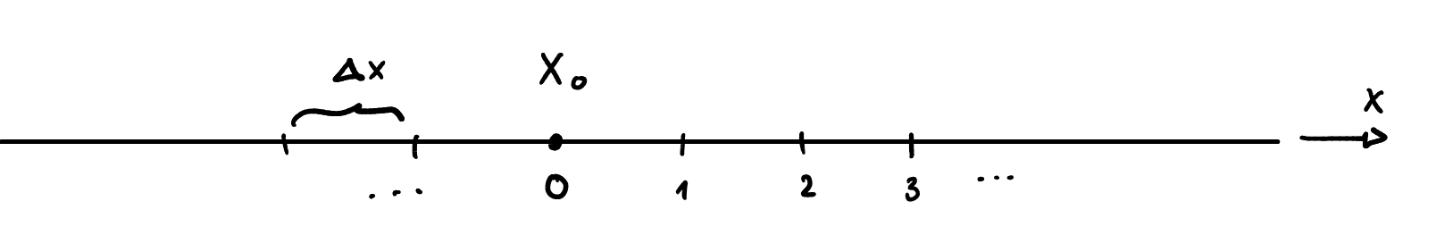
\includegraphics[width=0.7\linewidth]{Sketches/RandomWalk}
	%\caption{}
	\label{fig:randomwalk}
\end{figure}
we call $n(x,t)$ the number of particles at a position $x$ and time $t$ ("number density").

The change of $n$ in a time interval $\Delta t$ can be thought of as follows:

\begin{figure}[H]
	\centering
	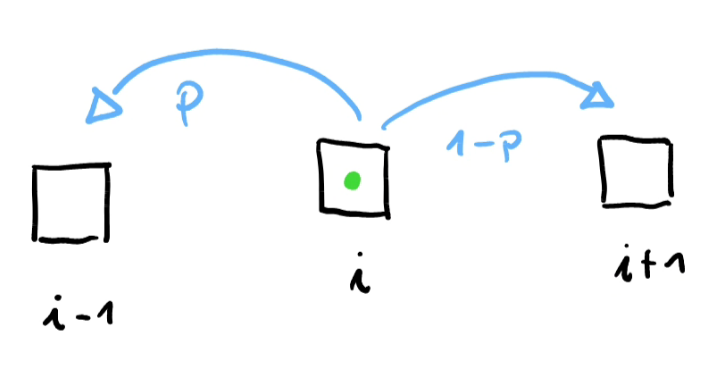
\includegraphics[width=0.3\linewidth]{Sketches/RandomWalkJumps}
	\caption{}
	\label{fig:randomwalkjumps}
\end{figure}

We assume that a particle jumps left with probability $p$ and towards the left with probability $1-p$. If $p=1/2$ we talk about an unbiased walk, when $p\ne 1/2$, it is a biased walk.

The change of particles in a time interval can be expressed as the outflow subtracted from the sum of influxes from the left and right:
\begin{equation}
	\Delta n \approx \frac{\partial n}{\partial t}\Delta t = n(x+\Delta x,t)p + n(x-\Delta x, t)(1-p)-n(x,t)
	\label{eq:diffusion_mass_conservation}
\end{equation}

This expression is just a discrete representation of mass conservation: No particle can get lost, they all have to go somewhere.

We treat $n(x,t)$ as continuous\footnote{Fishy, we know. This can also done by integrating formally to get a jump probability against time.} assuming that $\Delta x$s are really small and the amount of boxes is really large. We can therefore take a Taylor expansion:
\begin{equation*}
	\begin{split}
		n(x+\Delta x,t) = n(x)+\Delta x \frac{\partial n}{\partial x} + \frac{(\Delta x)^2}2 \frac{\partial ^2 n}{\partial x^2} + \dots \\
		n(x-\Delta x,t) = n(x)-\Delta x \frac{\partial n}{\partial x} + \frac{(\Delta x)^2}2 \frac{\partial ^2 n}{\partial x^2} + \dots \\
	\end{split}
\end{equation*}
which can be plugged into the equation \eqref{eq:diffusion_mass_conservation}:
\begin{equation*}
	\begin{split}
		\Delta n  &= \Delta x(p - (1-p))\frac{\partial n}{\partial x} + \frac{(\Delta x)^2}2\frac{\partial^2 n}{\partial x^2}+ \dots\\
		\frac{\partial n}{\partial t} &= -(1-2p)\frac{\Delta x}{\Delta t} \frac{\partial n}{\partial x} + \frac{(\Delta x)^2}{2\Delta t} \frac{\partial ^2 n}{\partial x^2}\qquad \left | \Delta x/ \Delta  t = v \right.\\
		\frac{\partial n}{\partial t} + v \frac{\partial n}{\partial x} &= D\frac{\partial ^2 n}{\partial x^2} \qquad \left | 
		\begin{cases}D = \frac{(\Delta x)^2}{2\Delta t} & \text{diffusion coefficient}\\ v=  (1-2p)\Delta x/\Delta t& \text{drift velocity}\end{cases}
		\right .
	\end{split}
\end{equation*}
For an unbiased random walk we pose $p=0.5$ which cancels the drift velocity. This makes the above turn into the well known Diffusion Equation:
\begin{equation}
	\boxed{\frac{\partial n}{\partial t} = D\frac{\partial ^2 n}{\partial x}}
	\label{eq:diffusion_1d}
\end{equation}
With the diffusion coefficient $D: [D]=m^2/s$

\paragraph{Remarks}
\begin{enumerate}
	\setlength{\itemsep}{-10pt}
	\item The net flux towards the left ($x+\Delta x \to x$) of an unbiased random walk is proportional to the gradient of the concentration $n$: $\frac 12 \Delta x \frac{\partial n}{\partial x} + \dots \propto \frac{\partial n}{\partial x}$.\\
	\item The same model applied for a 3D lattice yields a similar equation:$$\frac{\partial n}{\partial t}\ = D\nabla ^2n,\qquad D = \frac{\delta ^2}{6\Delta t}$$
	\item We can use this model to estimate diffusion coefficients: 
	\subitem Self diffusion: we know the velocity of a particle from statistical thermodynamics and can set $D \approx \frac \delta 6 \left(\frac{2k_b T}{m}\right)^{1/2}\approx 1.5\cdot 10^{-5} cm^2/s$ which is very exact.
	\subitem Suspended particles: A sphere of radius $a$ in a liquid with viscosity $\mu$ has a coefficient $D=\frac{k_BT}{6\pi \mu a}$, which is the Stokes-Einstein relation.
\end{enumerate}



\subsection{A Continuum Description of Diffusion}

We consider a concentration field $c(\vec x,t)$ of units $m^{-3}$. We start with the observation that molecules diffuse from higher to lower concentrations, which is expressed in \textbf{Fick's Law}:
\begin{equation}
	\vec j = -D\nabla c
	\label{eq:ficks_law}
\end{equation}

where $\vec j$ is the number flux: $\frac{1}{\mathrm{time}\cdot \mathrm{area}}$

\begin{figure}[H]
	\centering
	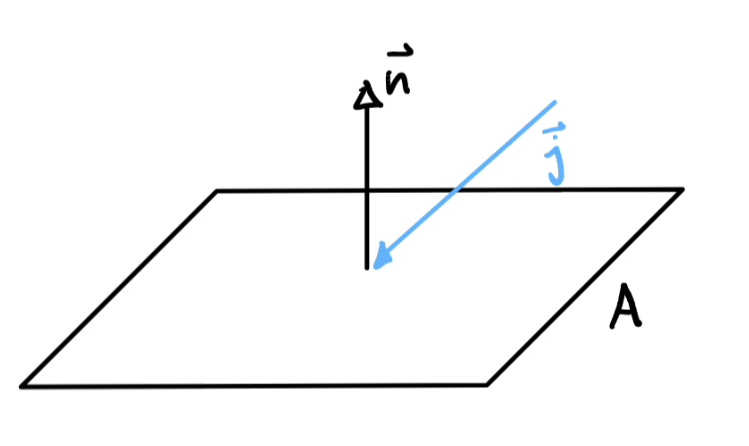
\includegraphics[width=0.3\linewidth]{Sketches/FicksLaw}
	%\caption{}
	\label{fig:fickslaw}
\end{figure}

The number of molecules transported trough area $A$ per time is
\begin{equation*}
	\int_A \vec j \cdot \hat n \, dA
\end{equation*}


Mass conservation in a control volume states, that the rate of change of "stuff" inside is the rate that goes out subtracted from the rate that goes in:
\begin{equation*}
	\begin{split}
	\frac \partial {\partial t}\left[\int_V c\,dV\right] &= -\oint_S \vec j \cdot \,d\vec S\\
	&\stackrel{(*)}{=} \int_V \nabla \cdot \vec j \,dV\\
	\int_V\frac{\partial c}{\partial t}\,dV &= -\int_V \nabla \cdot \vec j \,dV\\
	\int_V\frac{\partial c}{\partial t}- \nabla \cdot \vec j \,dV &= 0\\
	\end{split}
\end{equation*}
where at $(*)$ we used Gauss's law. The volume $V$ is arbitrary, so the above statement is true for all volumes $V$. This is only true, if the integrand is also zero. This leads to a representation of mass conservation in the general form of a differential conservation law:
\begin{equation*}
	\frac{\partial}{\partial t} c + \nabla \cdot \vec j = 0
\end{equation*}

Plugging in Fick's law ($\vec j = -D\nabla c$), we get
\begin{equation}
	\frac{\partial}{\partial t}c = \nabla (D\nabla c)
\end{equation}

For $D=const$ we get the diffusion equation from before:
\begin{equation}
	\boxed{\frac{\partial}{\partial t}c = D \nabla^2 c}
\end{equation}

\paragraph{Remarks} The equation results in \eqref{eq:diffusion_1d} in one dimension.









\setcounter{chapter}{4}
\renewcommand{\thechapter}{\arabic{chapter}}
